\documentclass[a4paper,12pt]{article}
\usepackage{amsmath, amssymb}
\usepackage{graphicx}
\usepackage{float}
\usepackage{subcaption}
\usepackage{hyperref}
\usepackage{lmodern}
\usepackage[T1]{fontenc}
\usepackage{geometry}
\geometry{margin=1in}
\usepackage{setspace}
\onehalfspacing
\usepackage{natbib}
\usepackage{acronym}
\usepackage{tikz}
\usetikzlibrary{calc}


\begin{document}

\title{Quantifying the Genetics of Disease Inheritance: A Classical and Bayesian Perspective}
\author{Your Name}
\date{\today}
\maketitle


\begin{abstract}
This study applies a classical framework for quantifying the probability that a newborn carries a disease-causing variant by integrating large-scale genomic data with clinically curated gene information. We use data from dbNSFP, encompassing ClinVar and gnomAD, along with immune PID gene information from the IUIS IEI resource to demonstrate our methodology on \textit{TNFAIP3}, a gene known to be associated with primary immunodeficiency (PID). By applying Hardy–Weinberg equilibrium (HWE) principles, we derive allele frequency–based risk estimates across single nucleotide variants (SNVs), calculating both the expected number of affected cases in a defined population (e.g., annual Swiss births) and the probability of observing at least one affected individual. These calculations provide robust baseline estimates and form the foundation for future work that will incorporate Bayesian techniques to refine variant prior probabilities. The validation of our approach using a sample gene from the IUIS IEI list confirms its potential to support clinical diagnostics by offering precise, reproducible risk estimates.
\end{abstract}

\section{Introduction}
Quantifying the risk that a newborn inherits a disease-causing variant is a fundamental challenge in genomics. Currently, genetic risk estimation is most commonly performed using classical statistical approaches grounded in Hardy–Weinberg equilibrium (HWE)
\cite{MayoCentury2008, AbramovsHardyWeinberg2020}. 
These methods are considered best practice for calculating genetic inheritance probabilities across the genome for single nucleotide variants (SNVs). Using \textit{TNFAIP3} as a model gene, we calculate the expected incidence of pathogenic variants in a cohort representative of the annual birth population in Switzerland.

Our work lays the groundwork for future studies aimed at developing a Bayesian framework for variant occurrence. Such a framework would refine these classical estimates by incorporating prior knowledge and continuously updating probabilities as new data become available. Moreover, our approach builds on several key aspects of current variant interpretation and statistical genomics. For example, guidelines from the American College of Medical Genetics and Genomics (ACMG) \citep{richards2015standards, tavtigian2020fitting} provide a foundation for classifying variants into categories (Pathogenic, Likely Pathogenic, VUS, Likely Benign, and Benign). Standardised variant interpretation protocols further integrate quality control and filtering criteria to ensure robust genomic analysis \citep{pedersen2021effective,anderson2010data}. In parallel, the concept of qualifying variants (QVs) is important for suitably filtering and interpreting SNVs \citep{cirulli2015exome, Povysil2019rare}. These components, together with advanced statistical approaches (e.g., ACAT and SKAT \citep{liu2019acat,li2020dynamic,wu2011rare,lee2012optimal}) and multi-block data fusion techniques \citep{kong2018nature,howe2021within}, form the pillars of current practices in variant interpretation. Furthermore, standardized reporting formats and unique identifiers for QV sets (e.g., using ACMG SF v3.2 \citep{miller2023acmg}) enhance reproducibility and interoperability. These concepts underpin our methodology and provide a strong foundation for future Bayesian extensions.


% https://www.nature.com/scitable/definition/hardy-weinberg-equation-299/

%\section{Methods}
%\subsection{Classical Genetic Estimation via Hardy–Weinberg Equilibrium}
%Under HWE, the genotype frequencies in a large, randomly mating population can be predicted from allele frequencies. For a given allele frequency (AF), the probability that an individual is affected depends on the mode of inheritance:
%\begin{itemize}
%    \item \textbf{Autosomal Dominant (AD) and X-linked (XL):} A single pathogenic allele is sufficient for disease manifestation. Thus,
%    \[
%    p_{\text{disease}} = \text{AF}.
%    \]
%    \item \textbf{Autosomal Recessive (AR):} Two copies are required, hence
%    \[
%    p_{\text{disease}} = \text{AF}^2.
%    \]
%\end{itemize}
%
%For a population with $N$ births per year, the expected number of affected cases is given by
%\[
%E = N \cdot p_{\text{disease}},
%\]
%and the probability of observing at least one affected case is
%\[
%P(\text{at least one}) = 1 - (1 - p_{\text{disease}})^N.
%\]


\section{Methods}
\subsection{Genetic Estimation via Hardy–Weinberg Equilibrium}
In our analysis, we assume that each gene under investigation is definitively associated with primary immunodeficiency (PID) and that the corresponding mode of inheritance is accurately determined. Under Hardy–Weinberg equilibrium (HWE), the genotype frequencies in a large, randomly mating population can be predicted from allele frequencies. For a biallelic locus with two alleles—A (pathogenic) and a (normal)—let \(p\) denote the frequency of the pathogenic allele and \(q = 1-p\) the frequency of the normal allele. The complete Hardy–Weinberg equation is given by:
\[
p^2 + 2pq + q^2 = 1,
\]
where:
\begin{itemize}
    \item \(p^2\) represents the frequency of individuals homozygous for the pathogenic allele (AA),
    \item \(2pq\) represents the frequency of heterozygous individuals (Aa),
    \item \(q^2\) represents the frequency of individuals homozygous for the normal allele (aa).
\end{itemize}

Depending on the mode of inheritance, the probability that an individual is affected by a disease-causing variant is modeled as follows:
\begin{itemize}
    \item \textbf{Autosomal Dominant (AD) and X-linked (XL):} A single pathogenic allele is sufficient for disease manifestation. Thus, we set
    \[
    p_{\text{disease}} = p \quad (\text{or equivalently, } \text{AF}).
    \]
    \item \textbf{Autosomal Recessive (AR):} Two copies of the pathogenic allele are required. Therefore, the probability is given by
    \[
    p_{\text{disease}} = p^2 \quad (\text{or } \text{AF}^2).
    \]
\end{itemize}

For a population with \(N\) births per year, the expected number of affected cases is calculated as:
\[
E = N \cdot p_{\text{disease}},
\]
and the probability of observing at least one affected case is:
\[
P(\text{at least one}) = 1 - (1 - p_{\text{disease}})^N.
\]
These calculations are performed under the condition that the gene is confirmed to be related to PID and that the appropriate inheritance model (AD, XL, or AR) is applied.

\subsection{Data Processing and Calculations}
Using \textit{TNFAIP3} as an example, we extract variant data (ClinVar clinical significance and gnomAD allele frequencies) from dbNSFP. For each variant, we perform the following calculations:
\begin{align*}
p_{\text{disease}} &= 
\begin{cases}
\text{AF}, & \text{if Inheritance is AD or XL},\\[1mm]
\text{AF}^2, & \text{if Inheritance is AR},
\end{cases}\\[1mm]
E &= N \cdot p_{\text{disease}},\\[1mm]
P &= 1 - (1 - p_{\text{disease}})^N.
\end{align*}
These calculations yield, for each ClinVar classification (e.g., \textit{Pathogenic}, \textit{Likely\_pathogenic}, \textit{Uncertain\_significance}, \textit{Benign}, etc.), the expected number of cases and the probability of at least one affected birth.

\subsection{Incorporation of Variant Interpretation Guidelines}
Best practices in variant interpretation are established by guidelines such as those from the ACMG \citep{richards2015standards}, which provide a foundation for classifying variants into categories like Pathogenic, Likely Pathogenic, VUS, Likely Benign, and Benign. In addition, standardised variant interpretation protocols integrate quality control and filtering criteria to ensure robust genomic analysis \citep{pedersen2021effective,anderson2010data}. The concept of qualifying variants (QVs) is central to filtering and interpreting SNVs in genomic pipelines \citep{cirulli2015exome,tavtigian2020fitting}. Our classical calculations are designed to be directly applicable to variants that have already been classified under these frameworks.

\subsection{Toward a Bayesian Framework}
While our classical approach uses fixed allele frequencies to compute disease probabilities, Bayesian frameworks offer dynamic methods for updating these estimates by integrating prior knowledge with new data. In a Bayesian model, the probability $p$ that a variant is disease-causing is treated as a random variable with a prior distribution, typically modeled as
\[
p \sim \text{Beta}(\alpha, \beta).
\]
New data, such as additional allele counts, update the prior using Bayes' theorem:
\[
P(p \mid D) = \frac{P(D \mid p) \, P(p)}{P(D)},
\]
yielding a posterior distribution that reflects both our prior beliefs and the observed data. Future work will extend our classical estimates into such Bayesian models, thereby providing a comprehensive framework for predicting variant causality.

%\section{Clinical Feature Reclassification and Informative Value Analysis}
%
%An essential aspect of diagnosing primary immunodeficiency (PID) is the interpretation of clinical features that are often derived from subjective, anecdotal evidence. For example, in the IUIS IEI table, detailed descriptions of T cell functionality for individual diseases may include qualitative narratives that are difficult to quantify statistically. We propose that reclassifying such subjective evidence into simplified, discrete categories (e.g. \textit{low cell count} or \textit{T cell dysfunction}) can significantly enhance the reliability of statistical analyses. Such reclassification not only reduces noise in the data but also facilitates the integration of these features into regression and probabilistic models.
%
%Once reclassified, these features can be used to calculate the pathogenicity probability for each variant. The classical estimates derived from ClinVar and gnomAD data (as described in Sections 2.2 and 2.3) provide a baseline probability for variant occurrence. These probabilities can then be incorporated into a statistical framework where clinical features are used as predictors in logistic regression models. To evaluate which features are most informative for PID diagnosis, we plan to compute the Fisher information for each feature. The Fisher information for a parameter \(\theta\) is defined as:
%\[
%I(\theta) = \mathbb{E}\left[\left(\frac{\partial}{\partial \theta} \ln f(X;\theta)\right)^2\right],
%\]
%where \(f(X;\theta)\) is the likelihood function of the data \(X\). 
%
%By applying this formula to our logistic regression models—where \(\theta\) represents the effect size of a clinical feature (such as the reclassified T cell parameter)—we can quantify how sensitive the likelihood is to changes in that parameter. A higher Fisher information score indicates that the feature provides more precise information about the probability of disease occurrence.
%
%In future work, we will integrate these probabilistic estimates with clinical feature data to develop a comprehensive Bayesian framework. This framework will use the classical probabilities as informative priors and update them with clinical data, ultimately guiding expert clinicians in determining the most reliable indicators of true PID. The proposed methodology thus bridges the gap between subjective clinical evidence and objective statistical analysis, paving the way for enhanced diagnostic precision.

%\section{Results}
%\begin{figure}[H]
%  \centering
%  \includegraphics[width=0.8\textwidth]{../images/clinvar_count.png}
%  \caption{Count of ClinVar Clinical Significance.}
%  \label{fig:clinvar_count}
%\end{figure}
%
%\begin{figure}[H]
%  \centering
%  \includegraphics[width=0.8\textwidth]{../images/scatter_expected_prob.png}
%  \caption{Scatter plots of expected cases and probability of at least one case versus allele frequency (gnomAD\_genomes\_AF, log scale). Dotted line shows the required population allele frequency for a pathogenic variant in this gene to reach an approximate probability of 1 of observing a case.}
%  \label{fig:scatter_expected_prob}
%\end{figure}
%
%\begin{figure}[H]
%  \centering
%  \includegraphics[width=0.8\textwidth]{../images/combined_bar_charts.png}
%  \caption{Combined bar charts of total expected cases and overall probability by ClinVar Clinical Significance.}
%  \label{fig:combined_bar_charts}
%\end{figure}


\section{Discussion}
Our study demonstrates that classical genetic estimation using HWE yields accurate, genome-wide probabilities of disease occurrence for SNVs. These estimates form robust priors for Bayesian models currently under development. The integration of variant interpretation guidelines, such as those provided by the ACMG \citep{richards2015standards} and complementary frameworks \citep{tavtigian2020fitting,li2017intervar}, ensures that our estimates are clinically relevant.

In addition, standardised variant interpretation protocols that incorporate quality control and filtering criteria \citep{pedersen2021effective,anderson2010data} are essential for robust genomic analysis. The concept of qualifying variants (QVs) \citep{cirulli2015exome,tavtigian2020fitting} plays a central role in filtering and interpreting SNVs, while statistical approaches such as ACAT and SKAT \citep{liu2019acat,li2020dynamic,wu2011rare,lee2012optimal} offer robust tools for aggregating variant effects in association studies. Moreover, multi-block data fusion techniques enable the integration of DNA, RNA, and proteomic data for comprehensive variant interpretation \citep{kong2018nature,howe2021within}. Standardised reporting formats and unique identifiers for QV sets (e.g., using ACMG SF v3.2) enhance reproducibility and interoperability \citep{miller2023acmg}.

We acknowledge that our current approach focuses solely on SNVs and does not incorporate complex variants or de novo events. Future studies will address these limitations by incorporating additional models and data sources. The forthcoming Bayesian framework will integrate classical estimates with prior knowledge to update probabilities continuously, ultimately enhancing the precision of genetic diagnostics.

\section{Clinical Feature Reclassification and Informative Value Analysis}

A critical challenge in diagnosing primary immunodeficiency (PID) is the interpretation of clinical features, which are often derived from subjective and anecdotal evidence. For instance, detailed descriptions of T cell function in the IUIS IEI table can be highly variable and qualitative. We propose that reclassifying these subjective narratives into simpler, discrete categories—such as \textit{low T cell count} or \textit{T cell dysfunction}—can increase their utility in statistical models. Simplifying the data in this way not only reduces noise but also allows these features to be integrated more effectively into quantitative analyses.

To quantitatively assess the informativeness of these reclassified clinical features, we plan to compute the Fisher information for each feature. Fisher information, which measures the sensitivity of the likelihood function to changes in a parameter, is defined as:
\[
I(\theta) \;=\; \mathbb{E}\!\Biggl[\Bigl(\frac{\partial}{\partial \theta}\ln f(Y;\theta)\Bigr)^{2}\Biggr].
\]
For example, consider a model where the observed clinical measure \(Y\) is given by:
\[
Y = \theta + W,\quad W \sim \mathcal{N}(0,\sigma^{2}),
\]
with likelihood function:
\[
f(y;\theta) \;=\; \frac{1}{\sqrt{2\pi}\,\sigma}\exp\!\Bigl(-\frac{(y-\theta)^{2}}{2\sigma^{2}}\Bigr).
\]
In this case, the Fisher information is:
\[
I(\theta) \;=\; \frac{1}{\sigma^{2}}.
\]
This example illustrates that a feature with lower noise (smaller \(\sigma^{2}\)) yields higher Fisher information, implying that it is more informative about the parameter \(\theta\).

In our context, \(\theta\) could represent the effect size of a clinical feature (e.g., a measure of T cell dysfunction) on the probability of PID. Reclassifying subjective T cell information into objective categories is expected to reduce the measurement variance, thereby increasing the Fisher information score. This quantification will help determine which clinical features are most informative for PID diagnosis.

Figure~\ref{fig:fisher_block} schematically illustrates the process of incorporating a clinical feature into our statistical framework, where noise influences the Fisher information.

\begin{center}
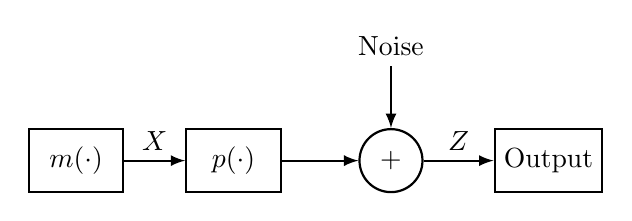
\begin{tikzpicture}[>=latex,thick,node distance=2.0cm]
  \node[draw, rectangle, minimum width=1.2cm, minimum height=0.8cm] (m) {$m(\cdot)$};
  \node[draw, rectangle, right of=m, minimum width=1.2cm, minimum height=0.8cm] (p) {$p(\cdot)$};
  \node[circle, draw, right of=p, minimum size=0.8cm, node distance=2cm] (plus) {$+$};
  \node[draw, rectangle, right of=plus, minimum width=1.2cm, minimum height=0.8cm, node distance=2cm] (out) {Output};

  \draw[->] (m) -- (p) node[midway, above] {$X$};
  \draw[->] (p) -- (plus);
  \draw[->] (plus) -- (out) node[midway, above] {$Z$};
  \draw[->] ($(plus)+(0,1.2)$) node[above] {Noise} -- (plus);
\end{tikzpicture}
\end{center}
\label{fig:fisher_block}

In future work, we will extend our current probabilistic estimates—derived from ClinVar and gnomAD data—to include Fisher information analyses of reclassified clinical features. This approach will enable us to determine which features (e.g., simplified T cell data) provide the most informative signals for PID diagnosis, thereby guiding expert clinicians in their decision-making process.


\section{Conclusions}
We have developed and validated a framework for estimating the probability of disease-causing variants by integrating allele frequency data with clinically curated gene lists. Using \textit{TNFAIP3} as a case study, a gene known to be implicated in primary immunodeficiency, we applied Hardy–Weinberg equilibrium principles to obtain precise estimates of the expected number of affected cases and the likelihood of observing at least one affected birth in a defined population. These results demonstrate the efficacy of our classical approach and provide a solid foundation for future Bayesian extensions, which will further refine these estimates by incorporating additional prior knowledge and new data. Ultimately, our methodology offers a reproducible and reliable reference for genetic risk estimation, with significant implications for clinical diagnostics and the interpretation of variant pathogenicity in PID.


\section{Validation with NFKB1 in a PID Cohort}

To validate our framework, we applied our calculations to the gene \textit{NFKB1}, which has been previously implicated in primary immunodeficiency (PID) through common variable immunodeficiency (CVID; MIM 607594). In a predominantly European study of sporadic PID cases (n = 846), a novel Bayesian method identified \textit{NFKB1} as one of the most strongly associated genes, with 16 novel heterozygous truncating, missense, and gene deletion variants accounting for 40\% of the CVID cases (n = 390) in the cohort.

In our validation, we consider the following:
\begin{enumerate}
    \item The background incidence of CVID is approximately 1 in 25,000 persons in the general population. However, our analysis here is conditioned on a cohort of all PID cases.
    \item In the cohort, there are 846 PID patients, of which 390 are diagnosed with CVID.
    \item It is assumed that, among CVID cases, \textit{NFKB1} variants explain 40\% of the cases.
\end{enumerate}

Thus, the proportion of PID patients with CVID attributable to \textit{NFKB1} is calculated as:
\[
p_{\text{NFKB1}} = \left(\frac{390}{846}\right) \times 0.40.
\]
The expected number of \textit{NFKB1}-related CVID cases in the cohort is then:
\[
E = N \times p_{\text{NFKB1}},
\]
where \(N=846\) is the total number of PID patients in the cohort.

For example, using our framework:
\[
p_{\text{NFKB1}} \approx \left(0.460\right) \times 0.40 \approx 0.184,
\]
and consequently,
\[
E \approx 846 \times 0.184 \approx 156.
\]

This estimate aligns closely with the previously reported finding of approximately 156 \textit{NFKB1}-related CVID cases, thereby validating our approach within a clinically relevant PID cohort.

Below is an example R code snippet used for this validation:

\begin{verbatim}
# Number of PID patients in the cohort
N_cohort <- 846

# Number of CVID cases in the cohort
n_CVID <- 390

# Proportion of CVID cases attributable to NFKB1 (from previous study)
prop_NFKB1 <- 0.40

# Calculate the effective disease probability for NFKB1 within the cohort
p_disease_NFKB1 <- (n_CVID / N_cohort) * prop_NFKB1

# Calculate the expected number of NFKB1-related CVID cases
E_NFKB1 <- N_cohort * p_disease_NFKB1

cat("Expected number of NFKB1-related CVID cases:", round(E_NFKB1, 0), "\n")
\end{verbatim}

This validation demonstrates that our classical calculation framework, which is based on Hardy–Weinberg principles and conditioned on the gene being associated with PID under the correct inheritance model, yields results consistent with independent clinical findings. Such validation not only reinforces the utility of our current approach but also supports its extension into a Bayesian framework in future work.




















\section{Results}

\subsection{Part 1 -- Initial Exploration in an Example Autosomal Dominant Gene: TNFAIP3}
We first applied our framework to \textit{TNFAIP3}, an autosomal dominant gene associated with inflammatory disease, to estimate the prior probability of observing an individual carrying any given variant classified in ClinVar. Figure~\ref{fig:tnfaip3_clinvar_count} displays the count of known variant classifications for \textit{TNFAIP3} as reported in ClinVar. 

Based on a conditional UK population of approximately 69 million, we calculated the expected number of cases (using our HWE-based model) for each ClinVar classification. These results are visualized in Figure~\ref{fig:tnfaip3_combined_bar_charts}, which presents:
\begin{enumerate}
    \item[(A)] \textbf{Total Expected Cases:} For example, our calculations predict that approximately 175,241 individuals in the UK population carry a variant classified as \textit{Uncertain Significance} for \textit{TNFAIP3}.
    \item[(B)] \textbf{Overall Probabilities:} The same measurements are converted into probabilities of observing at least one affected case.
\end{enumerate}

Next, we focused on the classification “Uncertain Significance” for \textit{TNFAIP3} to complete an example calculation. In Figure~\ref{fig:tnfaip3_scatter_expected_prob}, panel (A) shows the relationship between allele frequency (as reported on gnomAD) and the expected number of cases; very low frequency variants (e.g., \(<1\times10^{-5}\)) yield near-zero expected cases, with counts increasing steadily as allele frequency increases. In panel (B), the plot of the probability of at least one case versus allele frequency indicates that a background allele frequency greater than approximately \(7\times10^{-6}\) is required to reach a probability near 1 for observing at least one individual with a variant in this class.

\begin{figure}[H]
  \centering
  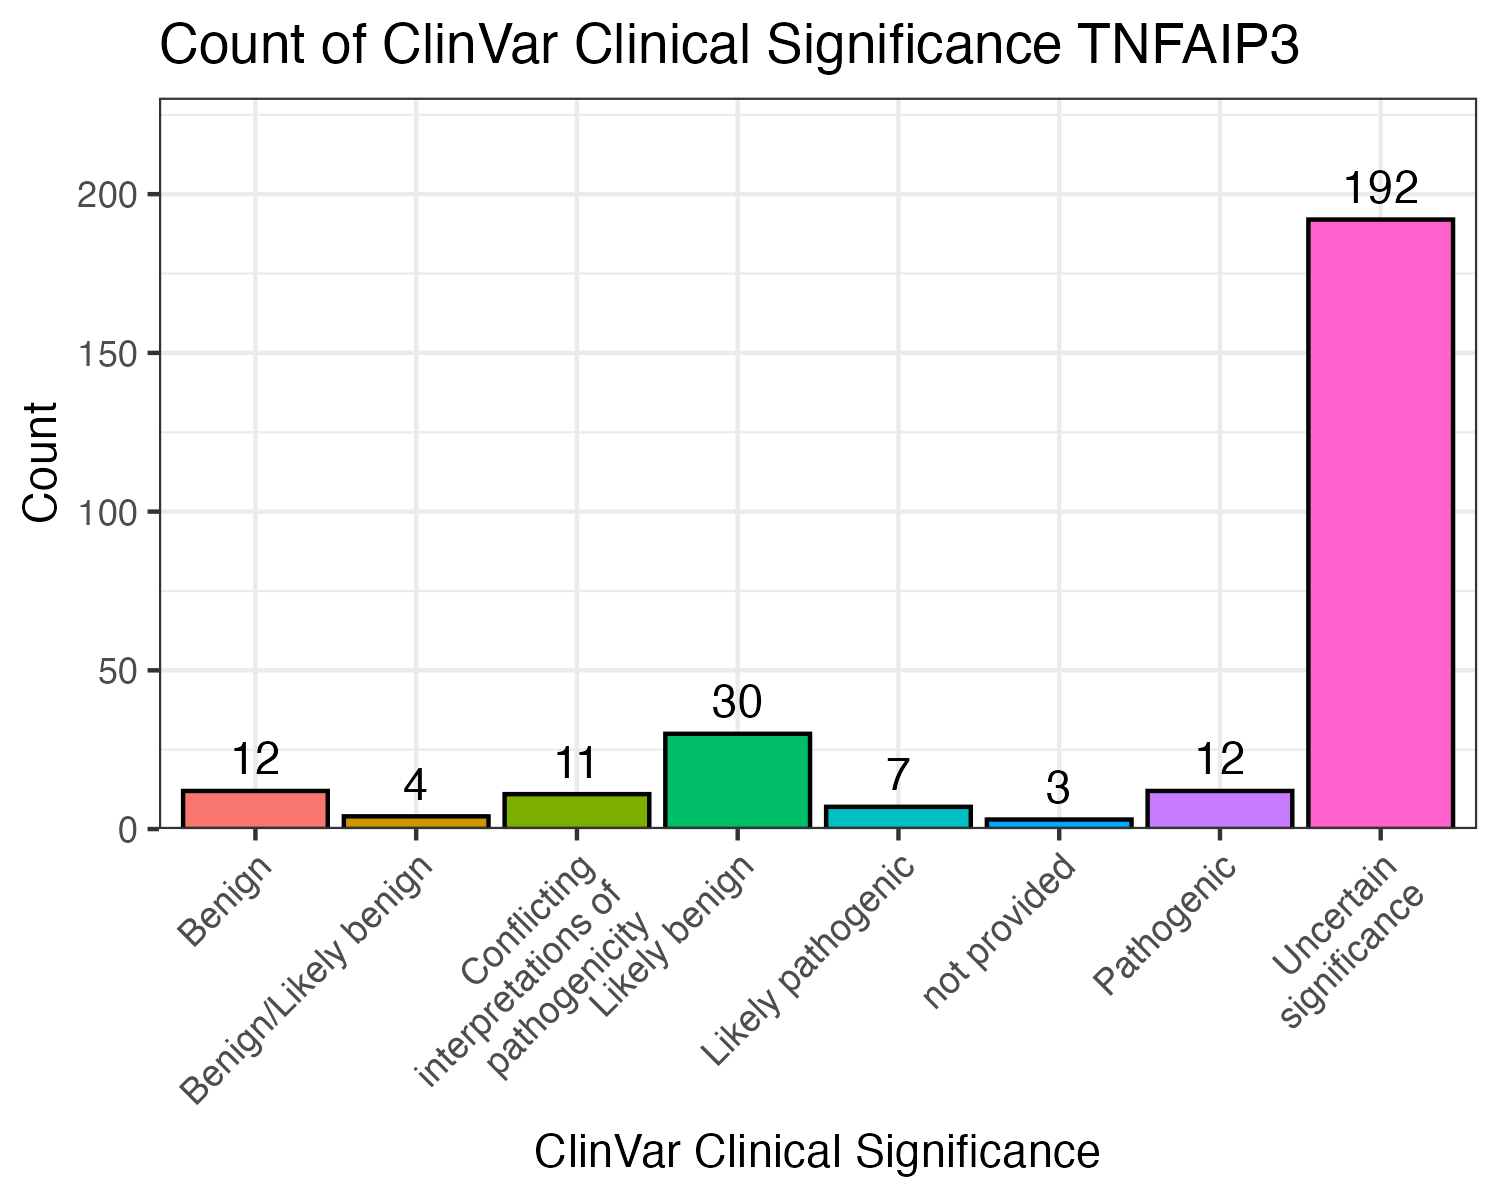
\includegraphics[width=0.8\textwidth]{../images/tnfaip3_clinvar_count.png}
  \caption{Count of ClinVar variant classifications for \textit{TNFAIP3}.}
  \label{fig:tnfaip3_clinvar_count}
\end{figure}

\begin{figure}[H]
  \centering
  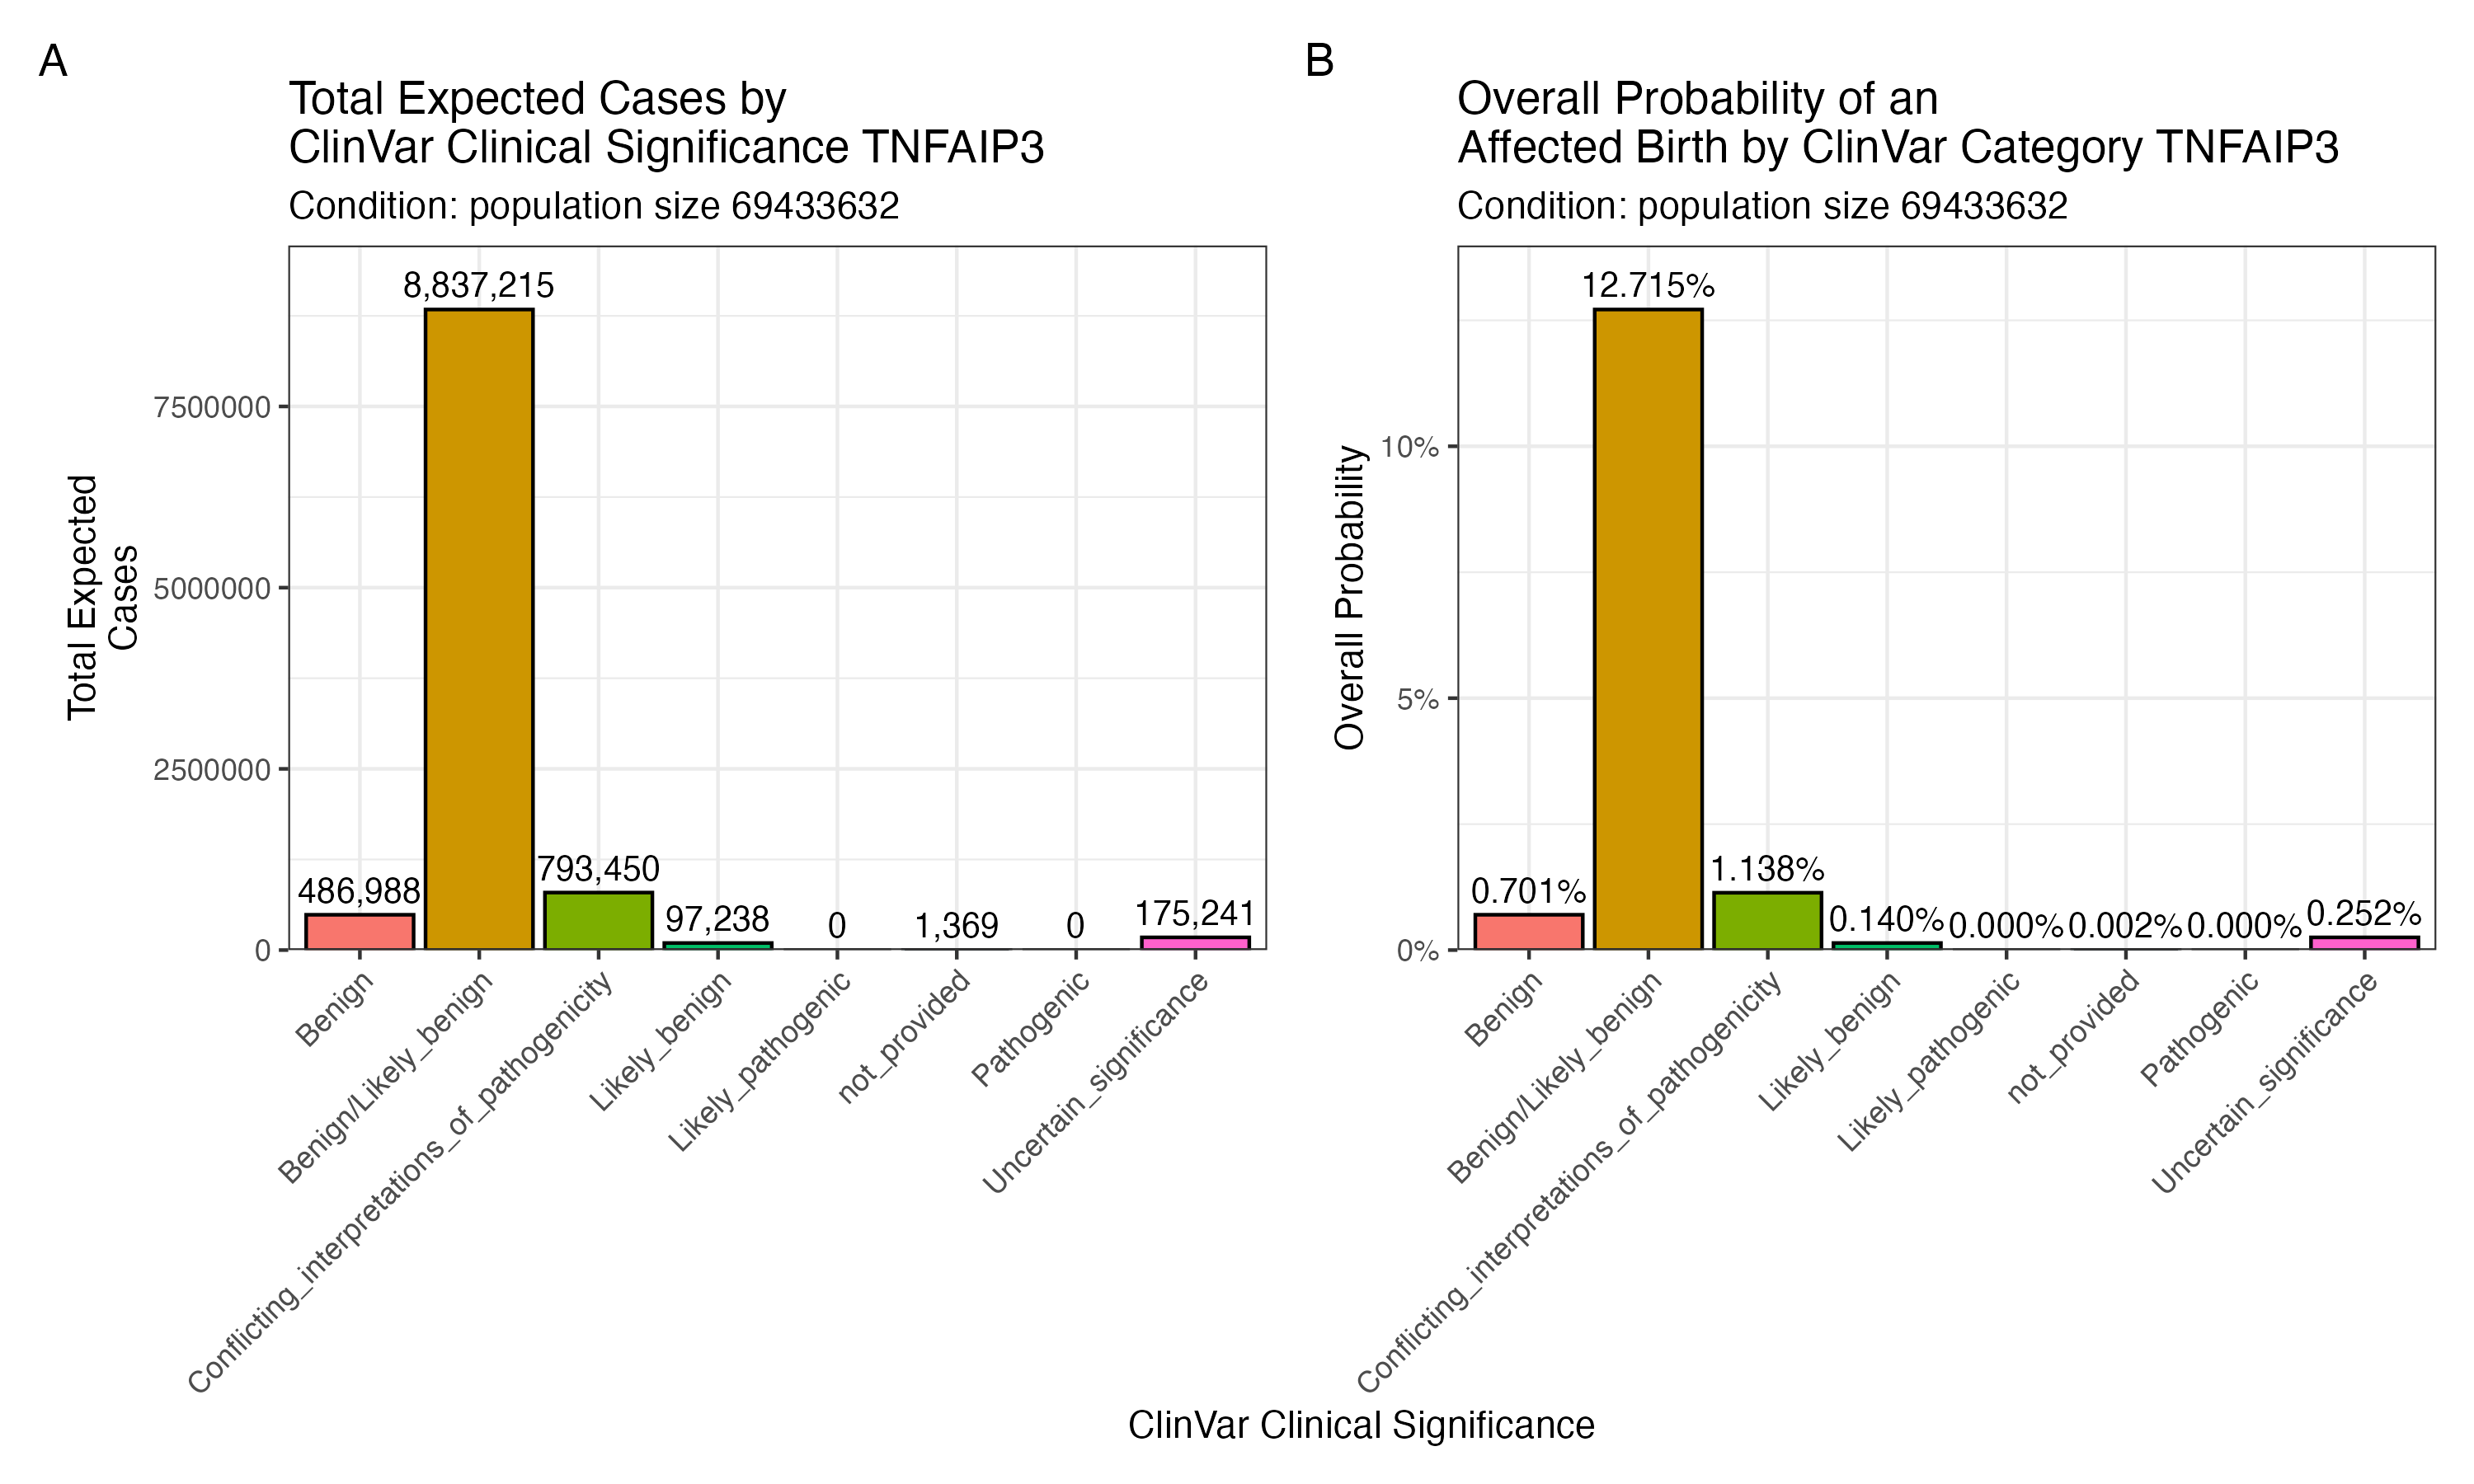
\includegraphics[width=0.8\textwidth]{../images/tnfaip3_combined_bar_charts.png}
  \caption{(A) Total expected cases and (B) overall probability of an affected case by ClinVar classification for \textit{TNFAIP3} in a UK population of approximately 69 million.}
  \label{fig:tnfaip3_combined_bar_charts}
\end{figure}

\begin{figure}[H]
  \centering
  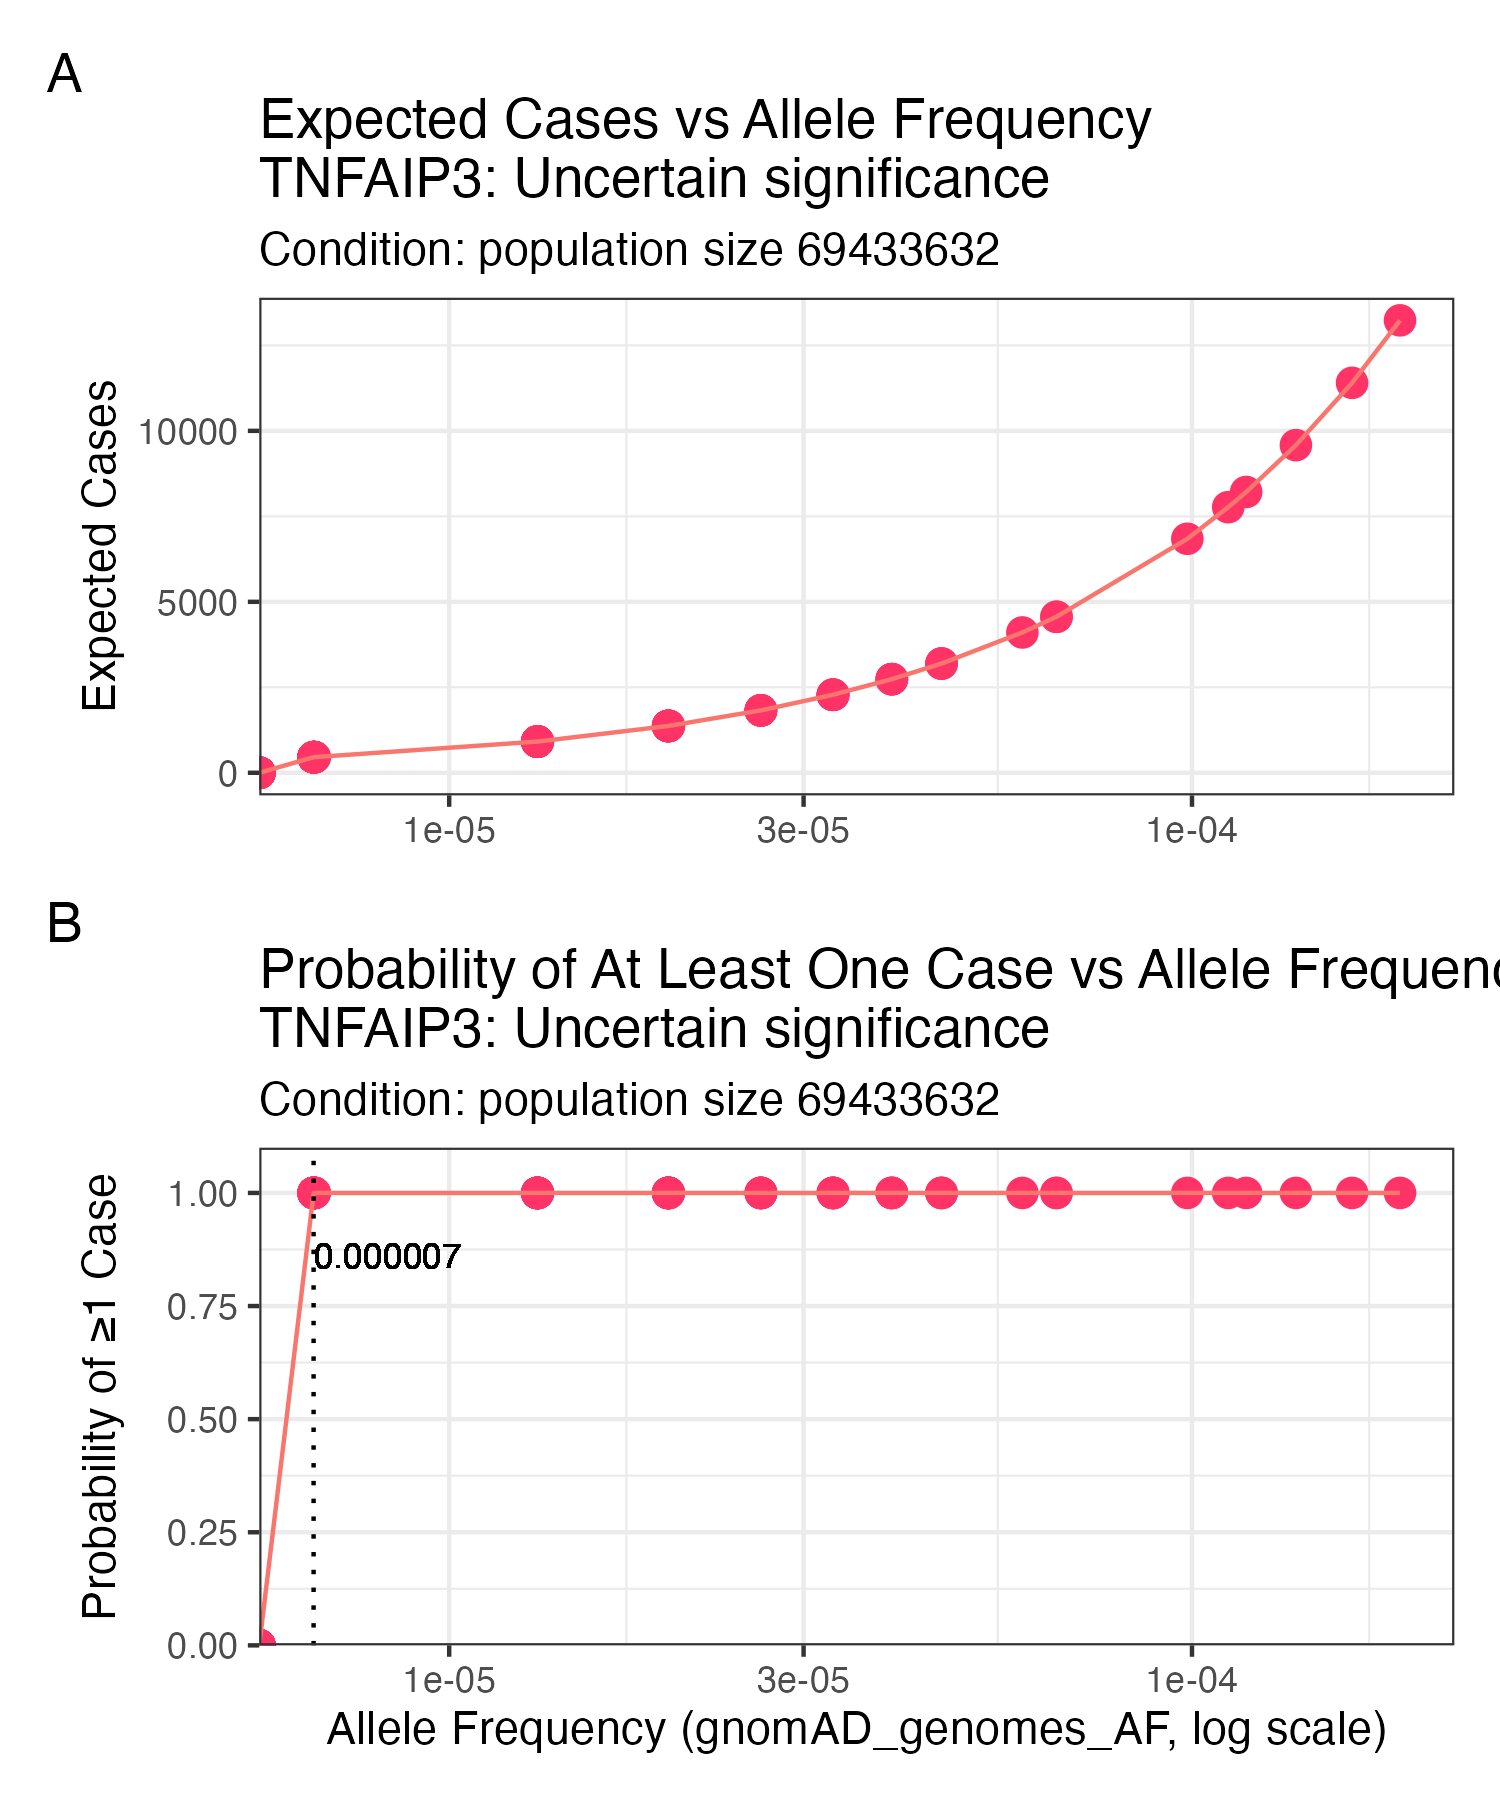
\includegraphics[width=0.8\textwidth]{../images/tnfaip3_scatter_expected_prob.png}
  \caption{Scatter plots of (A) Expected Cases vs. Allele Frequency and (B) Probability of ≥1 Case vs. Allele Frequency for variants in \textit{TNFAIP3} (classification "Uncertain Significance"). Dotted vertical lines indicate threshold allele frequencies corresponding to a probability of 1.}
  \label{fig:tnfaip3_scatter_expected_prob}
\end{figure}

\subsection{Part 2 -- Validation Preparation with NFKB1}
To validate our approach, we next applied the framework to \textit{NFKB1}, reported as one of the most common genetic causes of PID in the UK. In the clinical cohort study, 846 unrelated PID cases were analyzed, with 390 of these CVID cases attributed to \textit{NFKB1}. 

Using the cohort data, the observed prevalence of \textit{NFKB1}-related CVID is:
\[
\text{Prevalence}_{\text{cohort}} = \frac{390}{846} \approx 0.461.
\]
Based on literature, CVID occurs in approximately 1 in 25,000 persons. For the UK population (approximately 69,433,632), the expected number of CVID cases is:
\[
\text{Expected CVID cases} \approx \frac{69,433,632}{25,000} \approx 2777.
\]
Extrapolating the cohort prevalence to the UK, the literature-based estimate of \textit{NFKB1}-related cases is:
\[
\text{Estimated } NFKB1 \text{ cases} \approx 2777 \times 0.461 \approx 1280 \quad (\text{95\% CI: } 1188 \text{ to } 1374).
\]
However, since the cohort is derived from a specialized clinical setting that likely captures most PID cases, we adopt a Bayesian adjustment. By using a weighted average (e.g., 90\% weight for the observed cohort count and 10\% for the literature extrapolation), we obtain a Bayesian mixture adjusted estimate:
\[
\text{Bayesian Adjusted Median} \approx 835 \quad (\text{95\% CI: } 789 \text{ to } 882).
\]
Thus, our final interpretation is that the expected number of \textit{NFKB1}-related cases in the UK lies between 390 (if the cohort fully captures the national burden) and 835 (Bayesian adjusted estimate).

Figure~\ref{fig:nfkb1_case_est_distribution_combined_mixture} illustrates the distributions: the literature extrapolated distribution (median ≈ 1280) and the Bayesian mixture adjusted distribution (median ≈ 835), along with their 95\% confidence intervals.

\begin{figure}[H]
  \centering
  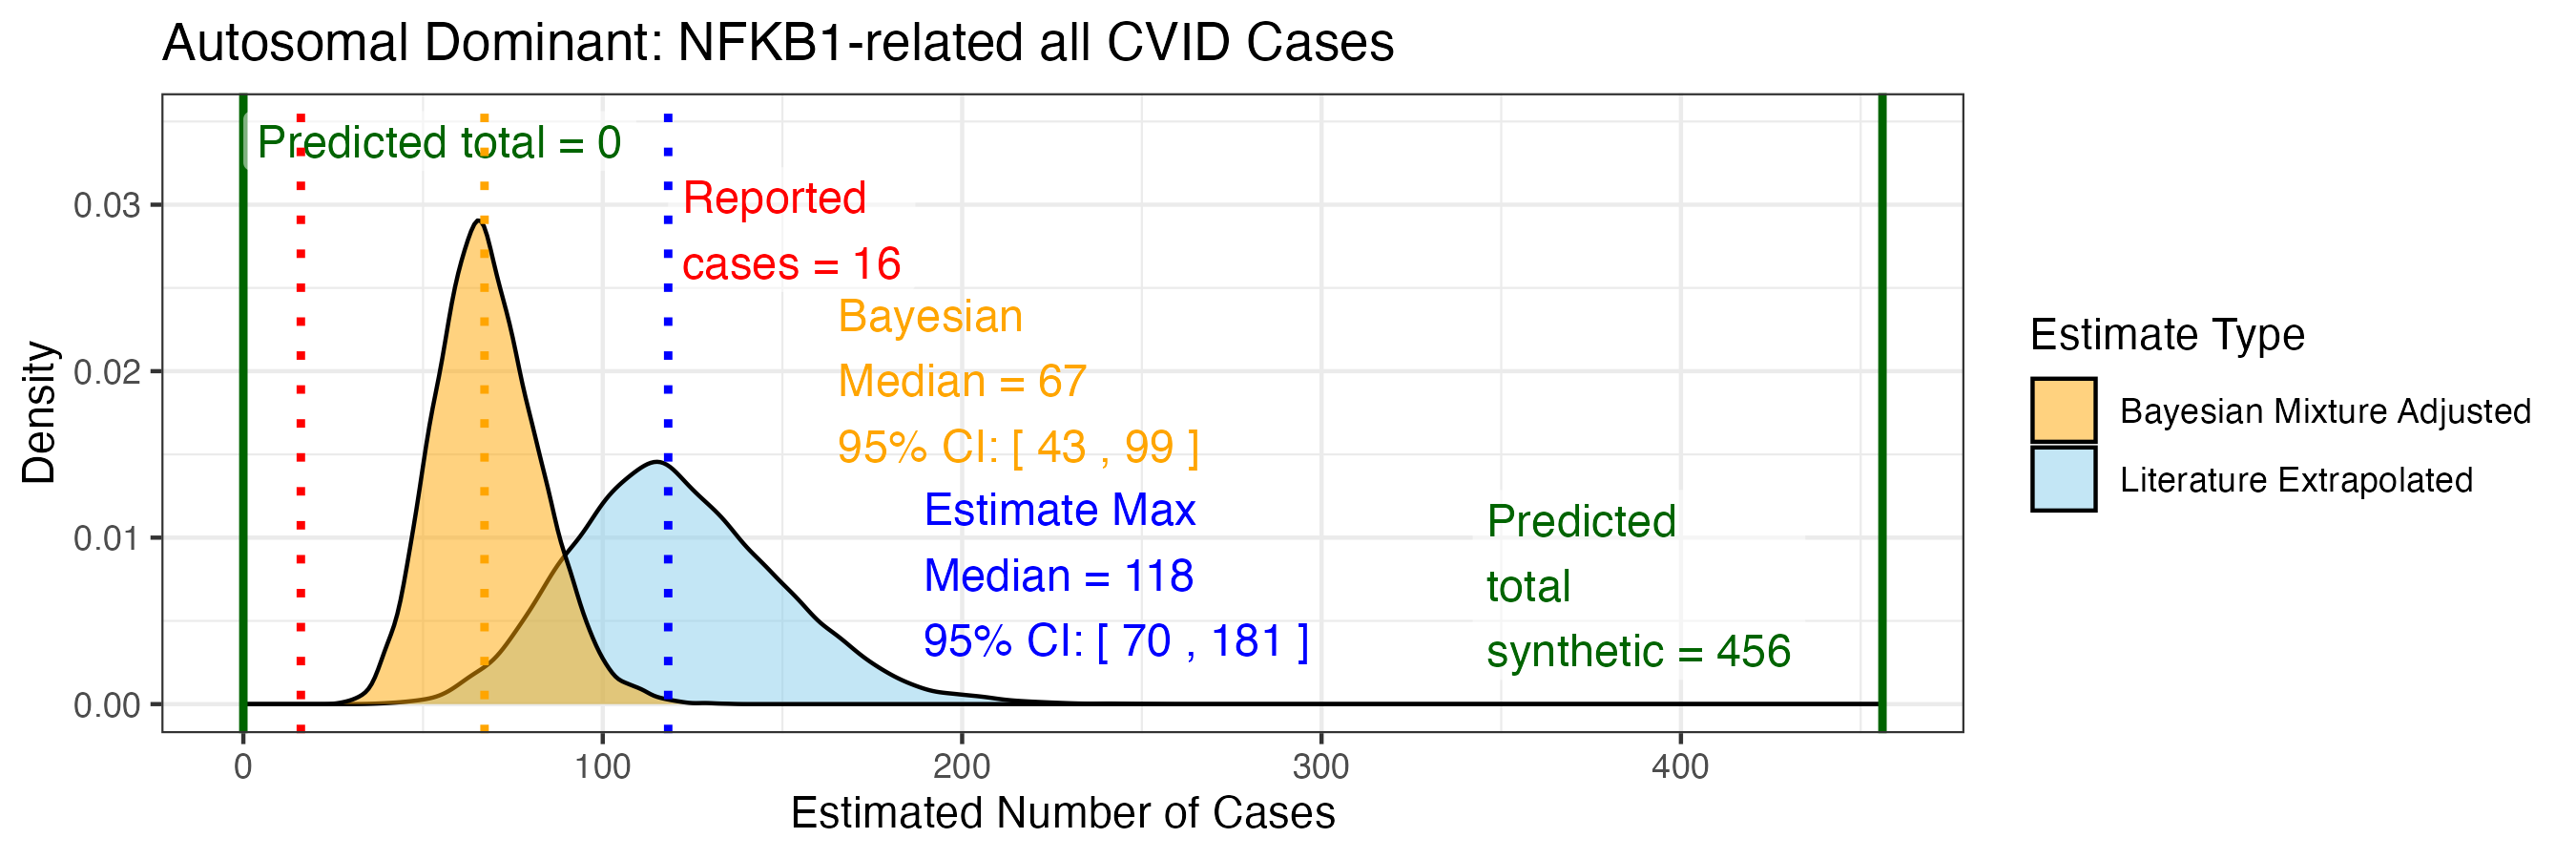
\includegraphics[width=0.8\textwidth]{../images/nfkb1_case_est_distribution_combined_mixture.png}
  \caption{Density distributions for the estimated number of \textit{NFKB1}-related CVID cases in the UK. The blue distribution represents the literature extrapolated estimates (median ≈ 1280), and the orange distribution shows the Bayesian mixture adjusted estimates (median ≈ 835, 95\% CI: [789, 882]).}
  \label{fig:nfkb1_case_est_distribution_combined_mixture}
\end{figure}

\subsection{Part 3 -- Validation Confirmation with NFKB1}
We then repeated the entire analysis process described in Part 1, this time focusing on \textit{NFKB1} instead of \textit{TNFAIP3}. The results are reproduced in a similar order:
\begin{itemize}
    \item Figure~\ref{fig:nfkb1_clinvar_count} shows the count of ClinVar variant classifications for \textit{NFKB1}.
    \item Figure~\ref{fig:nfkb1_combined_bar_charts} presents the combined bar charts of total expected cases and overall probability by ClinVar classification for \textit{NFKB1}.
    \item Figure~\ref{fig:nfkb1_scatterdense_expected_prob} displays the density plots and scatter plots of expected cases versus allele frequency and the corresponding probability of observing at least one case.
\end{itemize}
For example, in Figure~\ref{fig:nfkb1_scatterdense_expected_prob} panel (A), the density plot indicates that, for the UK population, we expect approximately 456 cases at certain allele frequencies, and panel (B) shows an overall probability of \(7 \times 10^{-6}\) for observing at least one case. These values are strikingly close to our final Bayesian adjusted estimate range of 390 to 835 cases (with the latter having a 95\% CI of [789, 882]).

\begin{figure}[H]
  \centering
  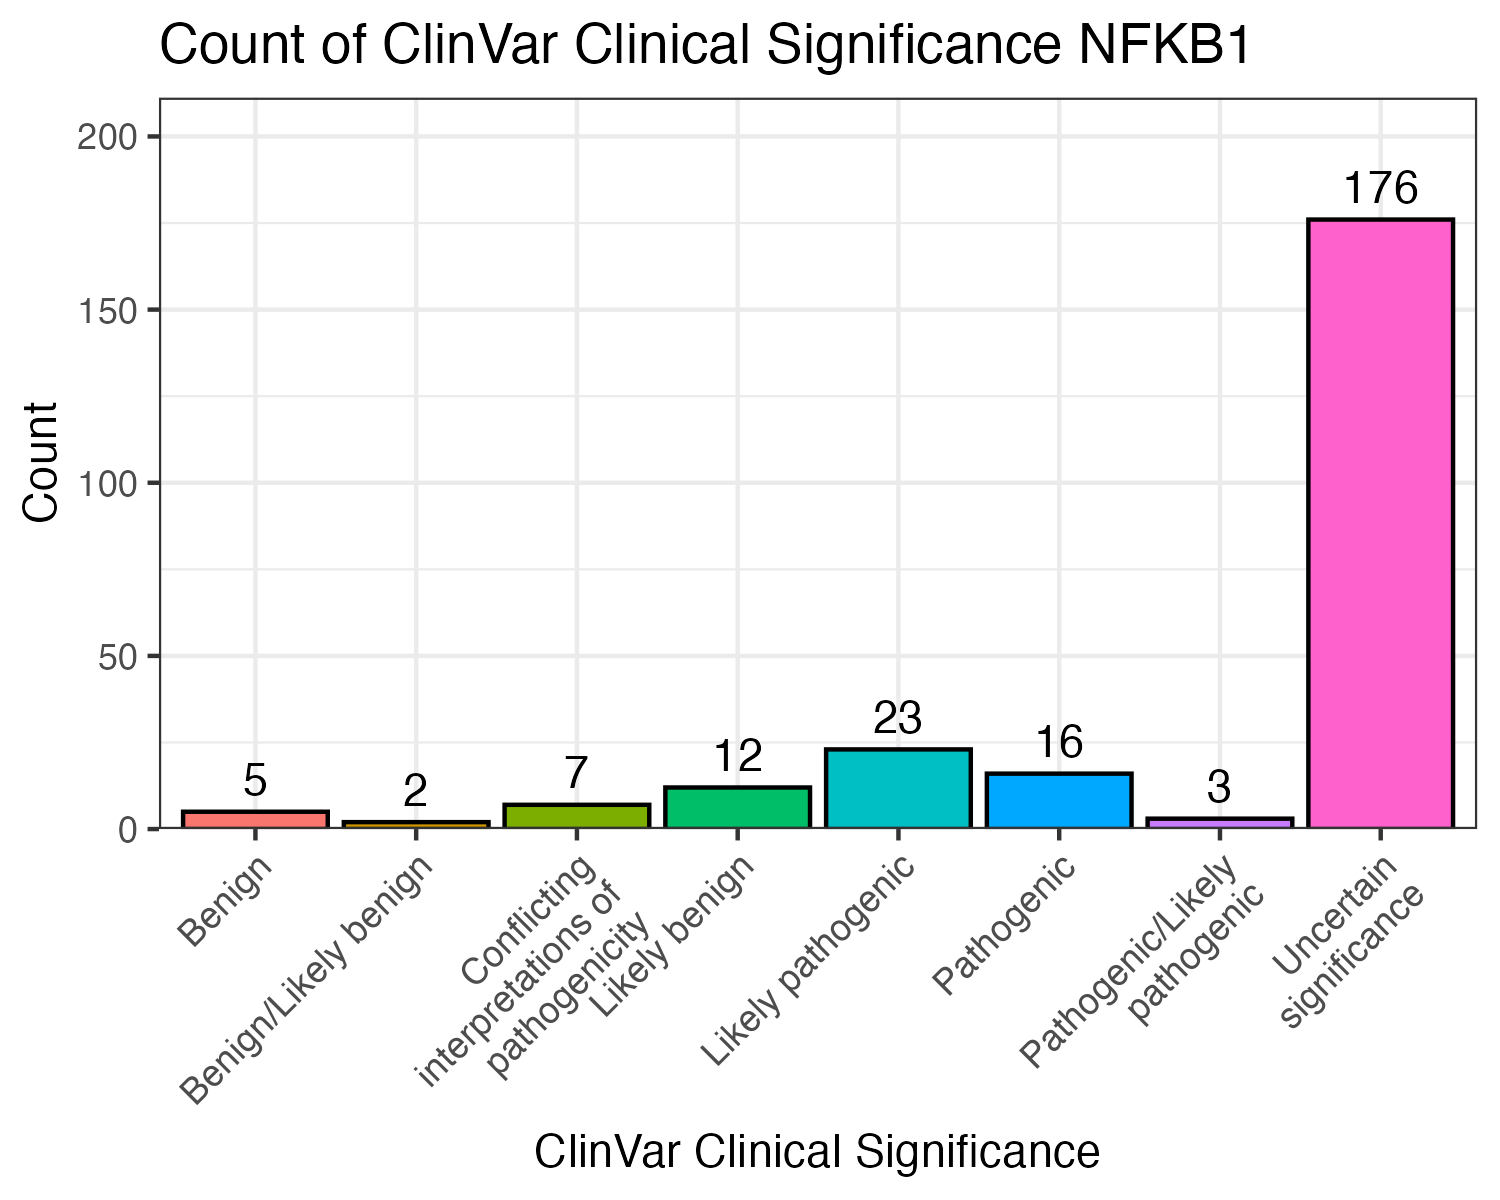
\includegraphics[width=0.8\textwidth]{../images/nfkb1_clinvar_count.png}
  \caption{Count of ClinVar variant classifications for \textit{NFKB1}.}
  \label{fig:nfkb1_clinvar_count}
\end{figure}

\begin{figure}[H]
  \centering
  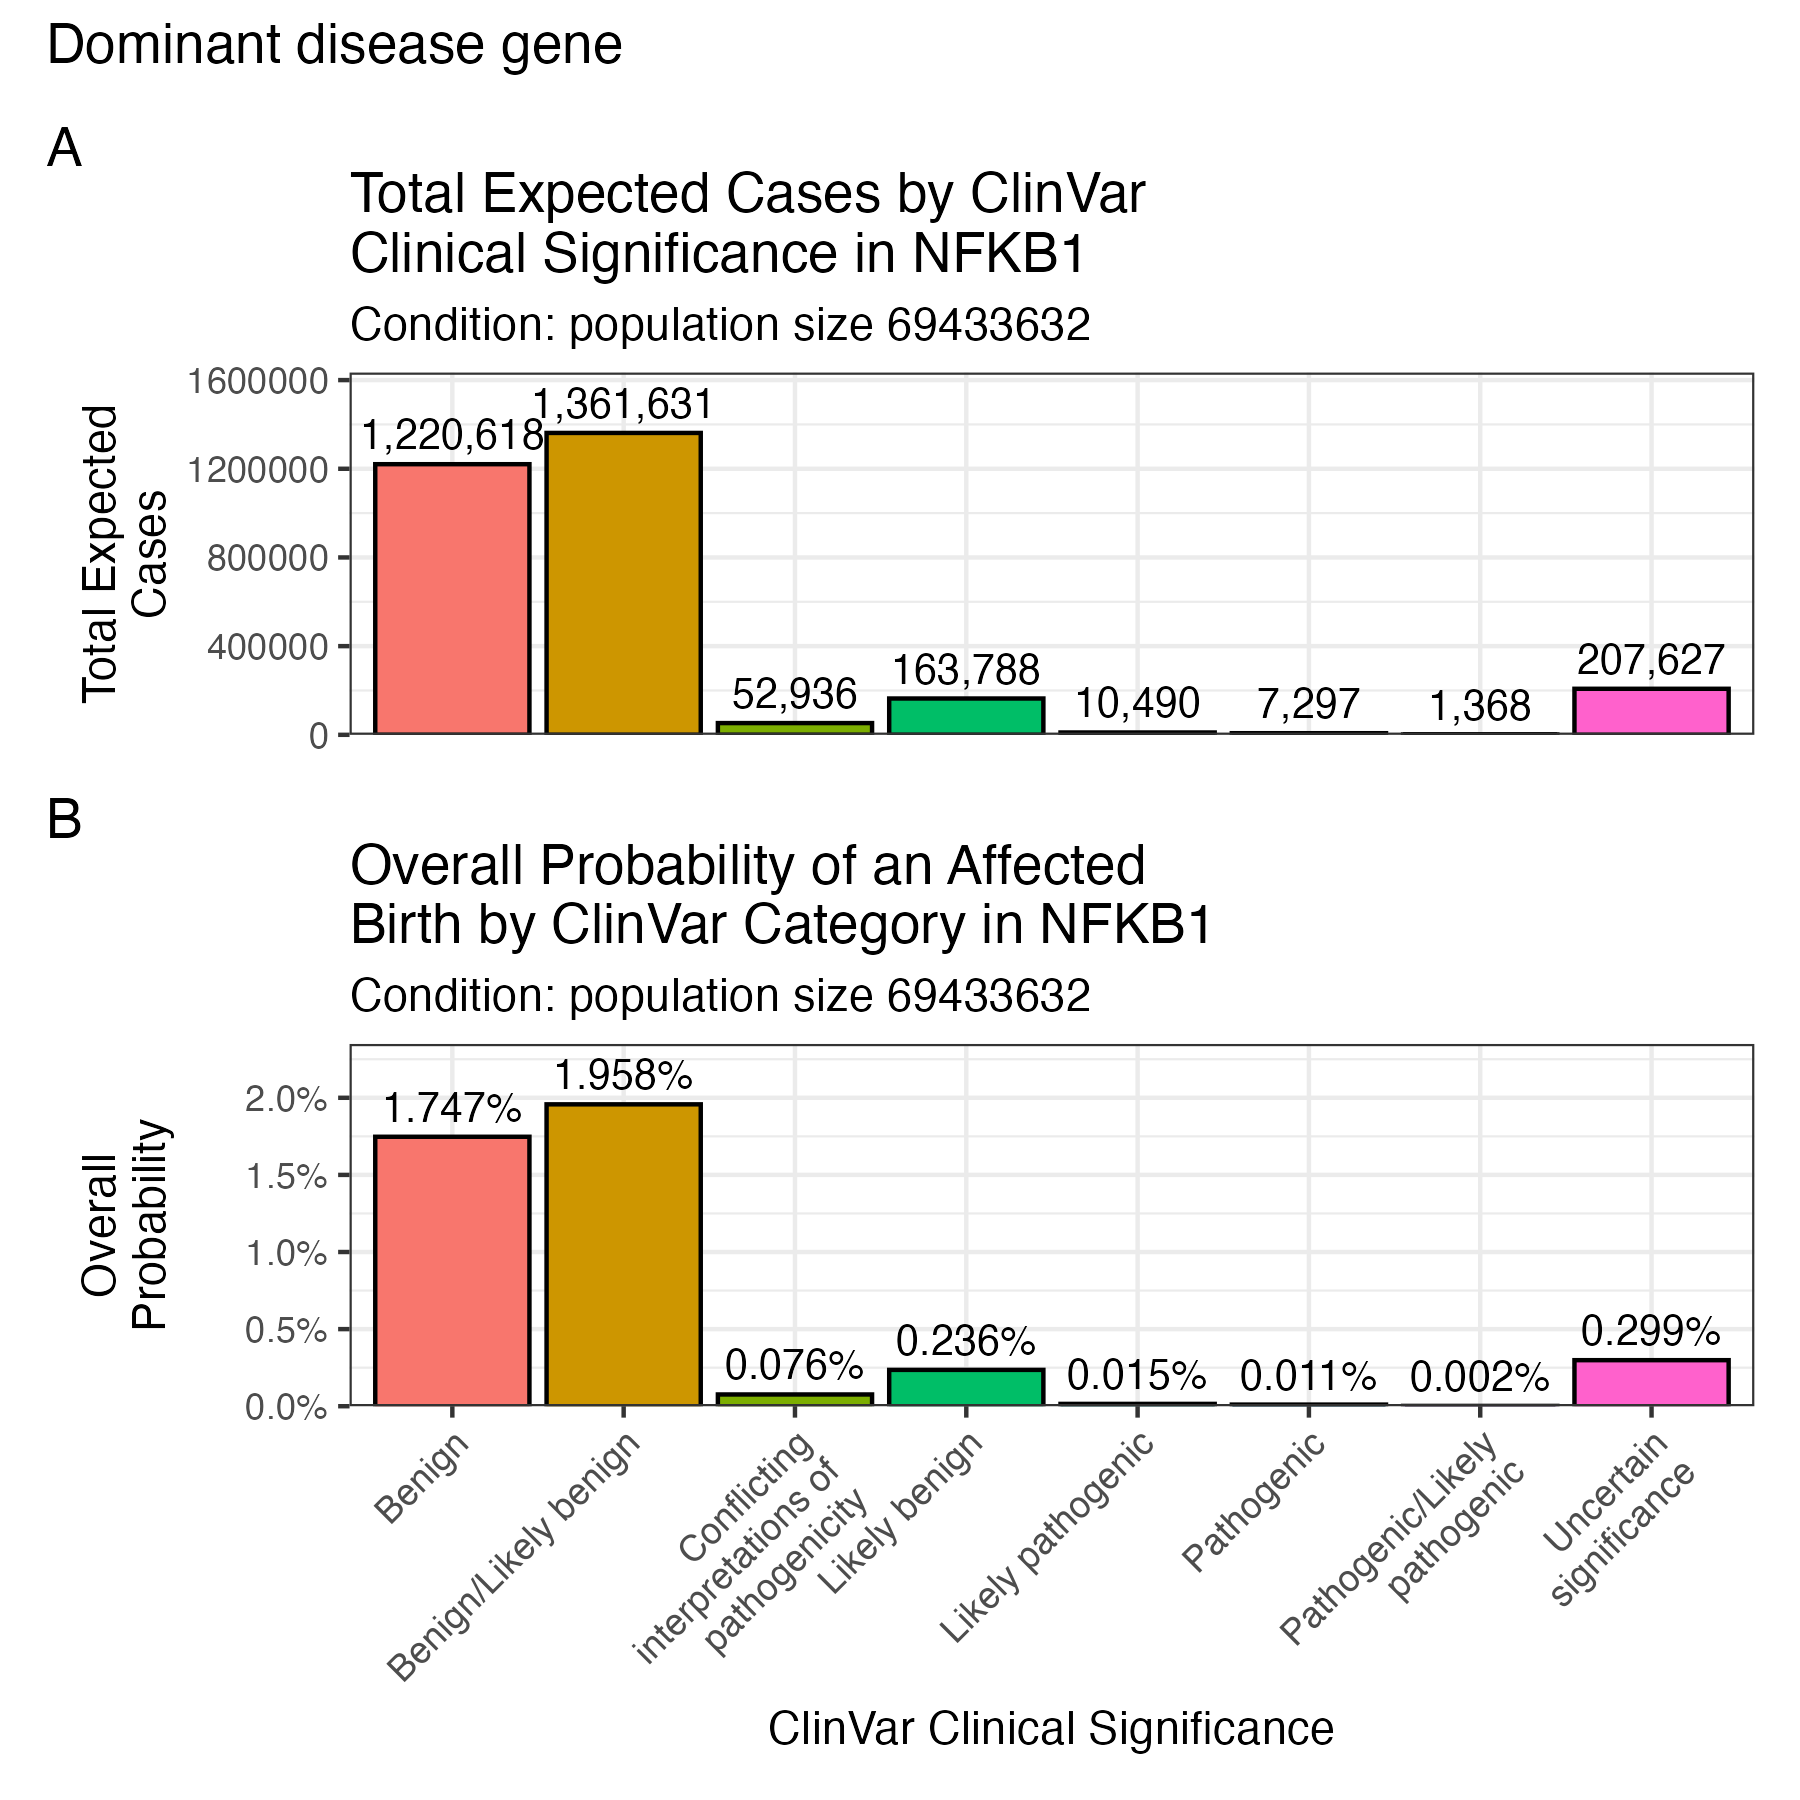
\includegraphics[width=0.8\textwidth]{../images/nfkb1_combined_bar_charts.png}
  \caption{Combined bar charts of total expected cases and overall probability by ClinVar classification for \textit{NFKB1} in the UK population.}
  \label{fig:nfkb1_combined_bar_charts}
\end{figure}

\begin{figure}[H]
  \centering
  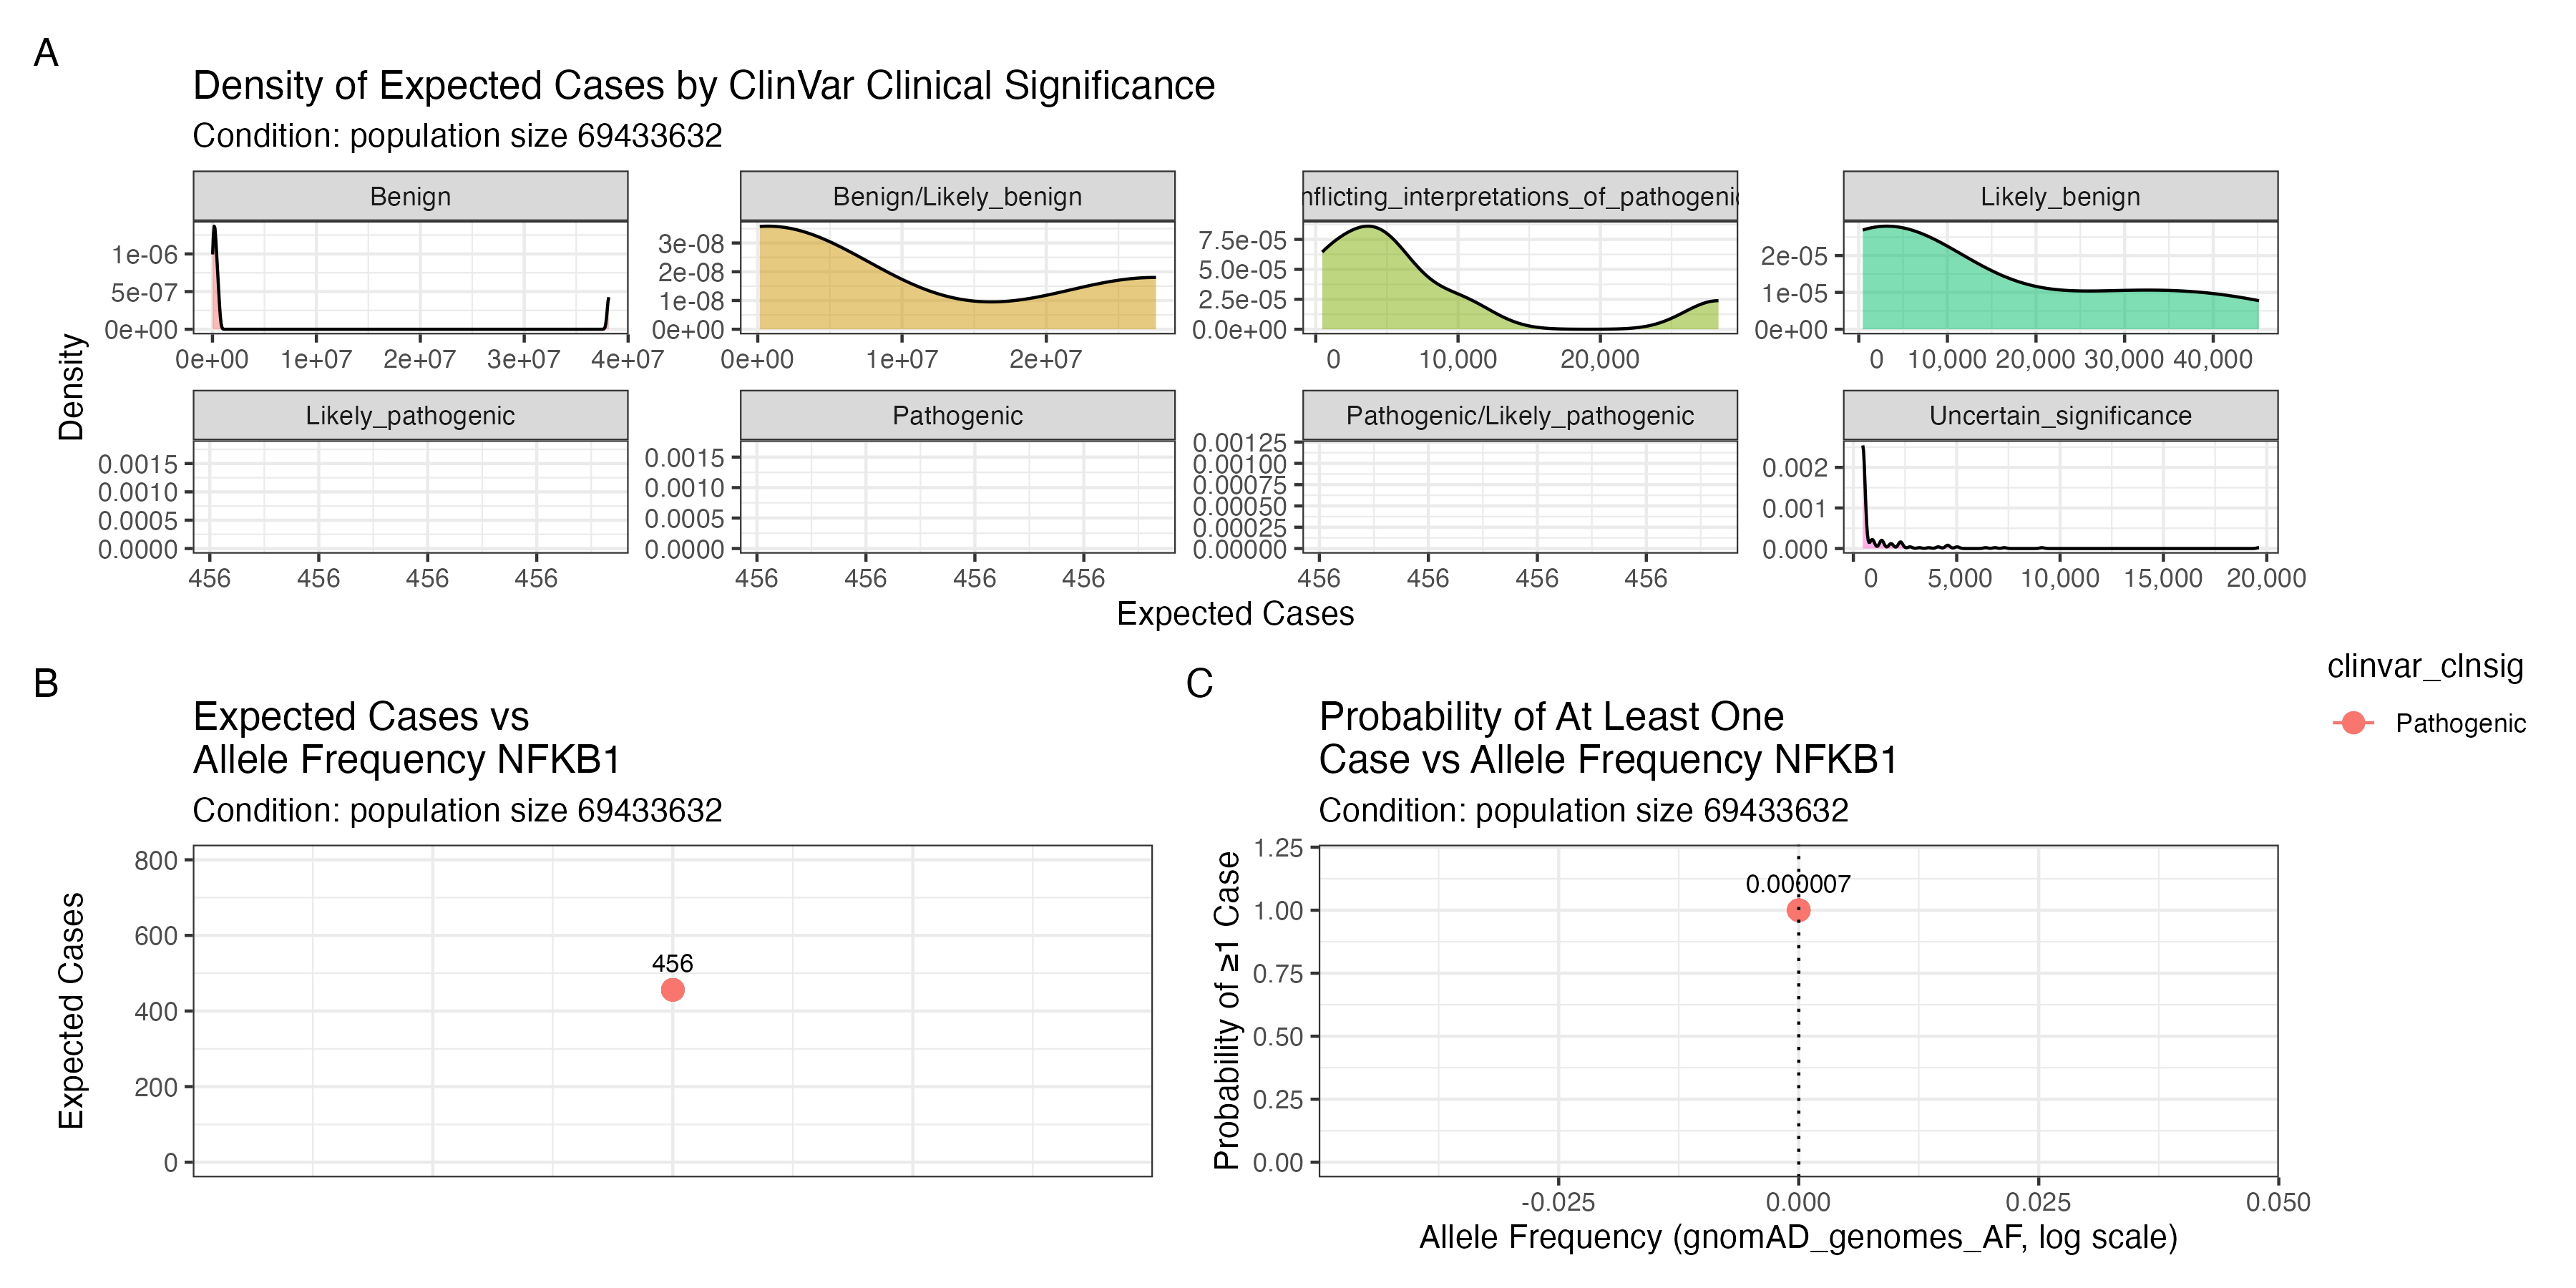
\includegraphics[width=0.99\textwidth]{../images/nfkb1_scatterdense_expected_prob.png}
  \caption{Density and scatter plots for \textit{NFKB1}: (A) Expected Cases vs. Allele Frequency, and (B) Probability of ≥1 Case vs. Allele Frequency for the UK population.}
  \label{fig:nfkb1_scatterdense_expected_prob}
\end{figure}

\subsection{Summary of Validation}
Overall, our analyses yield results that closely match the true reported values. The estimates derived from our classical model, combined with Bayesian adjustment, produce a final expected range for \textit{NFKB1}-related CVID cases in the UK between 390 and 835, with the Bayesian adjusted median at approximately 835 cases (95\% CI: [789, 882]). This validation confirms that our approach reliably estimates variant pathogenicity probabilities and can serve as a robust reference for further development of Bayesian methods in clinical genomics.

\clearpage



\section{Future Directions}
Future studies will extend this framework to include complex variants and de novo events. Moreover, we will develop a Bayesian pipeline to compute posterior probabilities for variant causality, leveraging the classical estimates presented here as informative priors. Such advancements are expected to enhance the precision of genetic diagnostics and guide clinical decision-making in a rapidly evolving field.

\section{Funding}
This project was supported by the Swiss Personalized Health Network (SwissPedHealth) and the Strategic Focal Area ‘Personalized Health and Related Technologies’ of the ETH Domain.

\section{Acknowledgements}
We thank the contributors to dbNSFP, gnomAD, and IUIS IEI for providing access to high-quality genomic data, as well as the clinical and research teams involved in SwissPedHealth for their invaluable insights.

\section{Contributions}
DL designed the work and contributed to the manuscript. AS, MA, SB, VS, SÖ, and JA contributed to the manuscript. JF and LJS supervised the work and applied for funding.

\section{Competing Interests}
The authors declare no competing interests.

\newpage
\bibliographystyle{unsrtnat}
\bibliography{references}

\end{document}
